\chapter{Power Architecture \& Circuit Safety}\label{ch:power}

\begin{tipbox}[When to Read This Chapter]
\textbf{Sprint~3}: Read the full chapter before CDR. The power budget, grounding strategy, and protection circuit sections directly determine whether your system will work reliably. \textbf{Sprint~4--5}: Return to the battery integration and EMI sections when debugging integration failures. \textbf{Related}: Circuit fundamentals in Chapter~13 (p.\,\pageref{ch:electronics}); motor/pump sizing in Chapter~11 (p.\,\pageref{ch:motors}); PCB implementation in Chapter~18 (p.\,\pageref{ch:pcb}); debugging ground loops in Chapter~20 (p.\,\pageref{ch:debug}).
\end{tipbox}

\vspace{1em}

Every electromechanical system needs a deliberately designed power architecture. A common student failure mode is treating power as an afterthought: ``I'll just wire everything to the battery.'' This leads to brown-outs, ground loops, component damage, and debugging sessions that consume entire sprints.

\begin{figure}[htbp]\centering
\begin{tikzpicture}[
    >=Stealth,prot/.style={rectangle, draw=WarnOrange, fill=WarnOrange!10,
        minimum width=1.4cm, minimum height=0.5cm, align=center,
        font=\tiny\sffamily, line width=0.5pt},
    arr/.style={->, line width=0.8pt, color=MinesBlue},
    gnd/.style={->, line width=0.6pt, color=diagGreen, densely dashed}
]
% Input stage
\node[block=MinesBlue] (src) at (0,0) {Power Source\\{\tiny Battery/Adapter}};
\node[prot] (rpol) at (2.3,0) {Reverse\\Polarity};
\node[prot] (fuse) at (4.2,0) {Main\\Fuse};
\node[prot] (tvs) at (6.0,0) {TVS\\Clamp};

% Regulation stage
\node[block=AccentTeal] (vreg1) at (8.5,1.2) {Buck 12\,V\\{\tiny Motor rail}};
\node[block=AccentTeal] (vreg2) at (8.5,0) {Buck 5\,V\\{\tiny Sensor rail}};
\node[block=AccentTeal] (vreg3) at (8.5,-1.2) {LDO 3.3\,V\\{\tiny MCU rail}};

% Distribution stage
\node[block=vbuild] (mot) at (12.0,1.2) {Motors\\{\tiny Per-motor fuse}};
\node[block=vbuild] (sen) at (12.0,0) {Sensors\\{\tiny Decoupled}};
\node[block=vbuild] (mcu) at (12.0,-1.2) {MCU\\{\tiny Decoupled}};

% Arrows
\draw[arr] (src) -- (rpol);
\draw[arr] (rpol) -- (fuse);
\draw[arr] (fuse) -- (tvs);
\draw[arr] (tvs) -| (vreg1.west);
\draw[arr] (tvs) -- (vreg2.west);
\draw[arr] (tvs) -| (vreg3.west);
\draw[arr] (vreg1) -- (mot);
\draw[arr] (vreg2) -- (sen);
\draw[arr] (vreg3) -- (mcu);

% Ground returns (dashed)
\draw[gnd] (mot.south) -- ++(0,-0.5) -| (0,-2.0);
\draw[gnd] (sen.south) -- ++(0,-0.7) -| (0,-2.0);
\draw[gnd] (mcu.south) -- ++(0,-0.9) -| (0,-2.0);
\node[font=\tiny\sffamily,diagGreen,fill=white,inner sep=1pt] at (8.0,-1.85) {Power GND};
\node[font=\tiny\sffamily,diagGreen,fill=white,inner sep=1pt] at (4.5,-2.15) {Signal GND};
\fill[diagGreen] (0,-2.0) circle (2pt);
\node[font=\tiny\sffamily\bfseries,diagGreen,left] at (-0.15,-2.0) {Star Point};

% Stage labels
\node[font=\tiny\sffamily,MinesSilver,above] at (3.1,0.7) {INPUT STAGE};
\node[font=\tiny\sffamily,MinesSilver,above] at (8.5,2.0) {REGULATION};
\node[font=\tiny\sffamily,MinesSilver,above] at (12.0,2.0) {DISTRIBUTION};
\end{tikzpicture}
\caption{Typical student project power architecture showing three stages: input protection (reverse polarity, fuse, TVS), regulation (cascaded converters from highest to lowest voltage), and distribution (per-load protection). Ground returns converge at a single star point near the source.}\label{fig:power_arch_tikz}
\end{figure}

\vspace{1em}


% ══════════════════════════════════════════════════════════════════════
\section{Power Architecture}
\label{sec:arch}
% ══════════════════════════════════════════════════════════════════════

\subsection{System-Level Design}

A well-designed power system (Figure~\ref{fig:power_arch_tikz}) flows from source through three functional stages before reaching the loads. The \textbf{input stage} is where power enters through a single, well-defined connector. This is where you place first-line protections: a keyed connector (prevents miswiring), reverse polarity protection, an input fuse, and a TVS diode for transient suppression. The \textbf{regulation stage} converts raw input voltage into the specific rails your system needs, commonly cascading from the highest voltage down (e.g., 24\,V input $\to$ 12\,V motor rail $\to$ 5\,V sensor rail $\to$ 3.3\,V MCU rail). The \textbf{distribution stage} delivers regulated power to each load through individual protection, per-rail fuses or electronic current limiters that prevent a fault in one subsystem from cascading.

\begin{figure}[htbp]
\centering
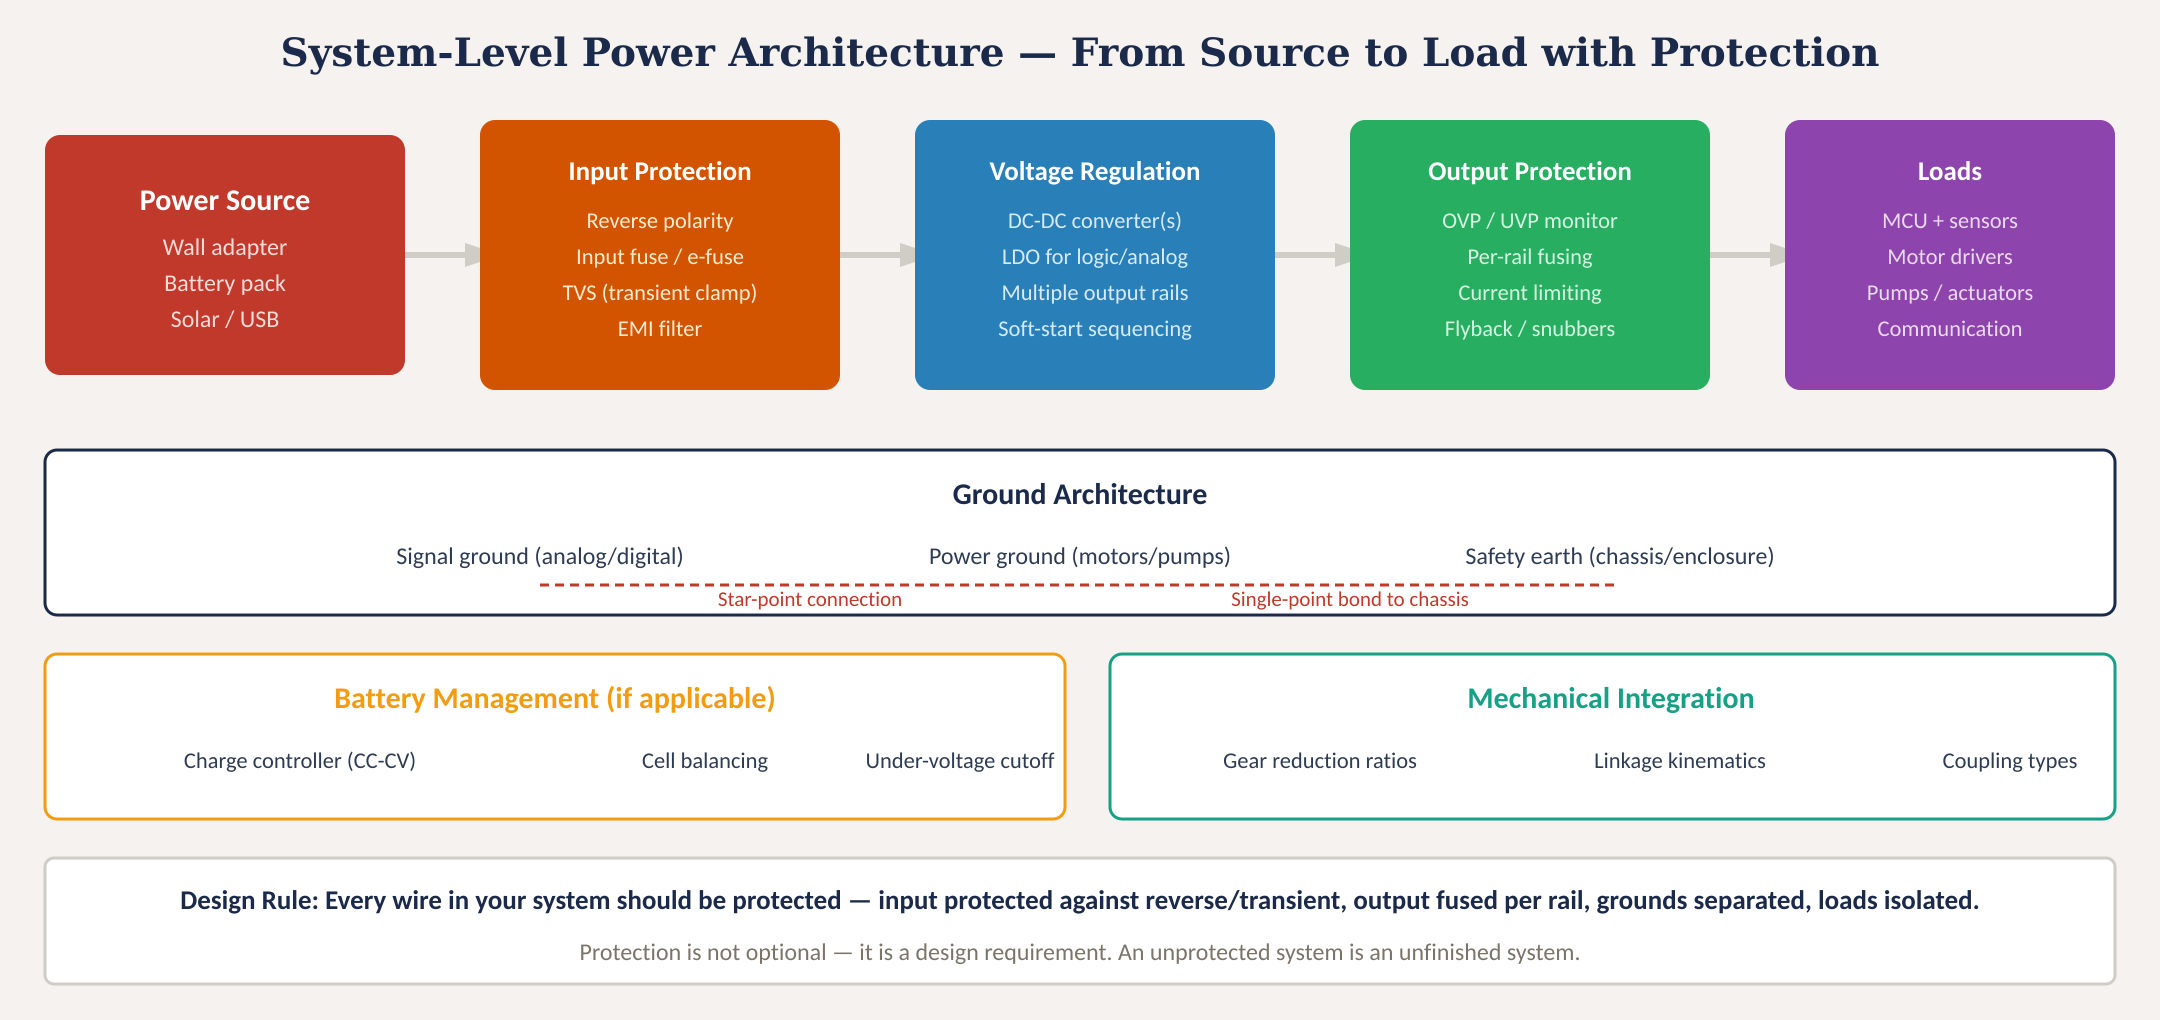
\includegraphics[width=\textwidth]{master_figs/fig_power_architecture.png}
\caption{System-level power architecture from source to load with protection stages, ground architecture, battery management, and mechanical integration.}
\label{fig:architecture}
\end{figure}

\subsection{Grounding Strategy}
\label{sec:grounding}

Ground is not a magical zero-volt reference; it is a real conductor with real resistance and inductance. When a motor draws 5\,A through a ground trace with 50\,m$\Omega$ resistance, there is a 250\,mV drop along that trace. If your ADC's ground reference shares that path, your sensor readings are corrupted.

\begin{keyconceptbox}[Star-Point Grounding\index{star-point grounding}]
Run separate ground conductors from each subsystem back to a single point near the power supply. Motor ground, sensor ground, and MCU ground each get their own conductor. They meet at \emph{one star point}. This prevents motor return current from flowing through sensor ground paths. See also Chapter~20 (p.\,\pageref{ch:debug}, Figure~\ref{fig:debug_flow}) for diagnosing ground-loop faults.
\end{keyconceptbox}

\subsubsection{Three Ground Domains}
\begin{itemize}[nosep,leftmargin=1.5em]
  \item \textbf{Signal ground}: analog sensors, ADCs, digital logic. Low current, noise-sensitive.
  \item \textbf{Power ground}: motors, pumps, solenoids, heaters. High current, noisy.
  \item \textbf{Safety earth}: metal enclosure, chassis. Fault-current path for AC-powered systems.
\end{itemize}

\begin{warningbox}[The \#1 Debugging Time Sink]
Poor grounding is the single most common cause of difficult-to-diagnose intermittent failures in student projects. If your sensor readings are noisy, your MCU resets when a motor starts, or your serial communication drops characters; check your grounding first.
\end{warningbox}

\begin{warningbox}[AC Mains Safety]
Use a Class~II (double-insulated) wall adapter whenever possible; no earth ground connection is needed. If you must use an internal open-frame supply, bond the metal enclosure to earth ground through a 3-prong inlet with proper strain relief. \textbf{Never defeat a ground prong.} AC mains voltage (120\,V/240\,V) is lethal. All AC wiring must use appropriately rated wire, fuses, and enclosures. If your project requires AC mains wiring, consult with the instructor before proceeding.
\end{warningbox}

\subsubsection{Signal Isolation}
Use optocouplers or digital isolators (Si8620, ADUM1201) to pass signals between high-voltage and low-voltage domains. Essential when controlling AC loads (relays, triacs) from a microcontroller.


\subsection{Battery Integration}
\label{sec:battery}

Lithium cells (LiPo, Li-ion, LiFePO\textsubscript{4}) store enormous energy density and can cause fire or explosion if mishandled. A Battery Management System (BMS) is \textbf{mandatory}:

\begin{itemize}[nosep,leftmargin=1.5em]
  \item Overcharge cutoff: 4.2\,V/cell maximum.
  \item Deep-discharge cutoff: 3.0\,V/cell minimum (irreversible damage below this).
  \item Overcurrent / short-circuit shutoff.
  \item Cell balancing for multi-cell packs.
\end{itemize}

Common modules: TP4056 (single-cell charger, CC-CV profile), BQ25895 (buck-boost charger IC), BQ76940 (multi-cell BMS). During development, always store and charge lithium batteries in a fireproof LiPo-safe bag. \textbf{Never charge unattended without a BMS.}

\begin{tipbox}[DC Generation Sources (Solar, Alternator)]
Solar panels produce variable voltage; use an MPPT charge controller to extract maximum power. Always include a blocking diode to prevent battery discharge through the panel at night. For alternators: rectify the AC output, regulate with a charge controller, and add TVS/MOV protection against load-dump voltage spikes if the battery disconnects while the alternator is running.
\end{tipbox}


% ══════════════════════════════════════════════════════════════════════

\subsection{Power Budget Spreadsheet: How to Build One}
The power budget is a spreadsheet with one row per component and the following columns:

\begin{table}[htbp]\centering\small
\begin{tabularx}{\textwidth}{l l c c c X}
\toprule
\textbf{Component} & \textbf{Rail} & \textbf{$I_{typ}$ (mA)} & \textbf{$I_{peak}$ (mA)} & \textbf{Duty (\%)} & \textbf{$I_{avg}$ (mA)} \\
\midrule
ESP32 (active) & 3.3V & 80 & 240 & 10 & 8.0 \\
ESP32 (deep sleep) & 3.3V & 0.01 & --- & 90 & 0.009 \\
DS18B20 sensor & 3.3V & 1.5 & 1.5 & 100 & 1.5 \\
SIM7000G (TX) & 4.0V & 200 & 2000 & 1 & 2.0 \\
Relay coil & 12V & 80 & 80 & 5 & 4.0 \\
\midrule
\multicolumn{4}{l}{\textbf{3.3V rail total}} & & \textbf{9.5} \\
\multicolumn{4}{l}{\textbf{3.3V rail peak}} & & \textbf{241.5} \\
\multicolumn{4}{l}{\textbf{12V rail total}} & & \textbf{4.0} \\
\bottomrule
\end{tabularx}
\caption{GreenShield power budget example.}
\end{table}

The peak column sizes your regulators and fuses. The average column sizes your battery. Add 25\% margin to both. If the SIM7000G's 2\,A peak on the 4\,V rail shares a regulator with the ESP32, that regulator must handle 2.24\,A peak; a common sizing mistake.

\section{Protection Circuits}
\label{sec:protection}
% ══════════════════════════════════════════════════════════════════════

The philosophy is \textbf{defense in depth}: layer multiple protections so that each catches what the previous one missed. No single device guards against all threats.

\begin{figure}[htbp]
\centering
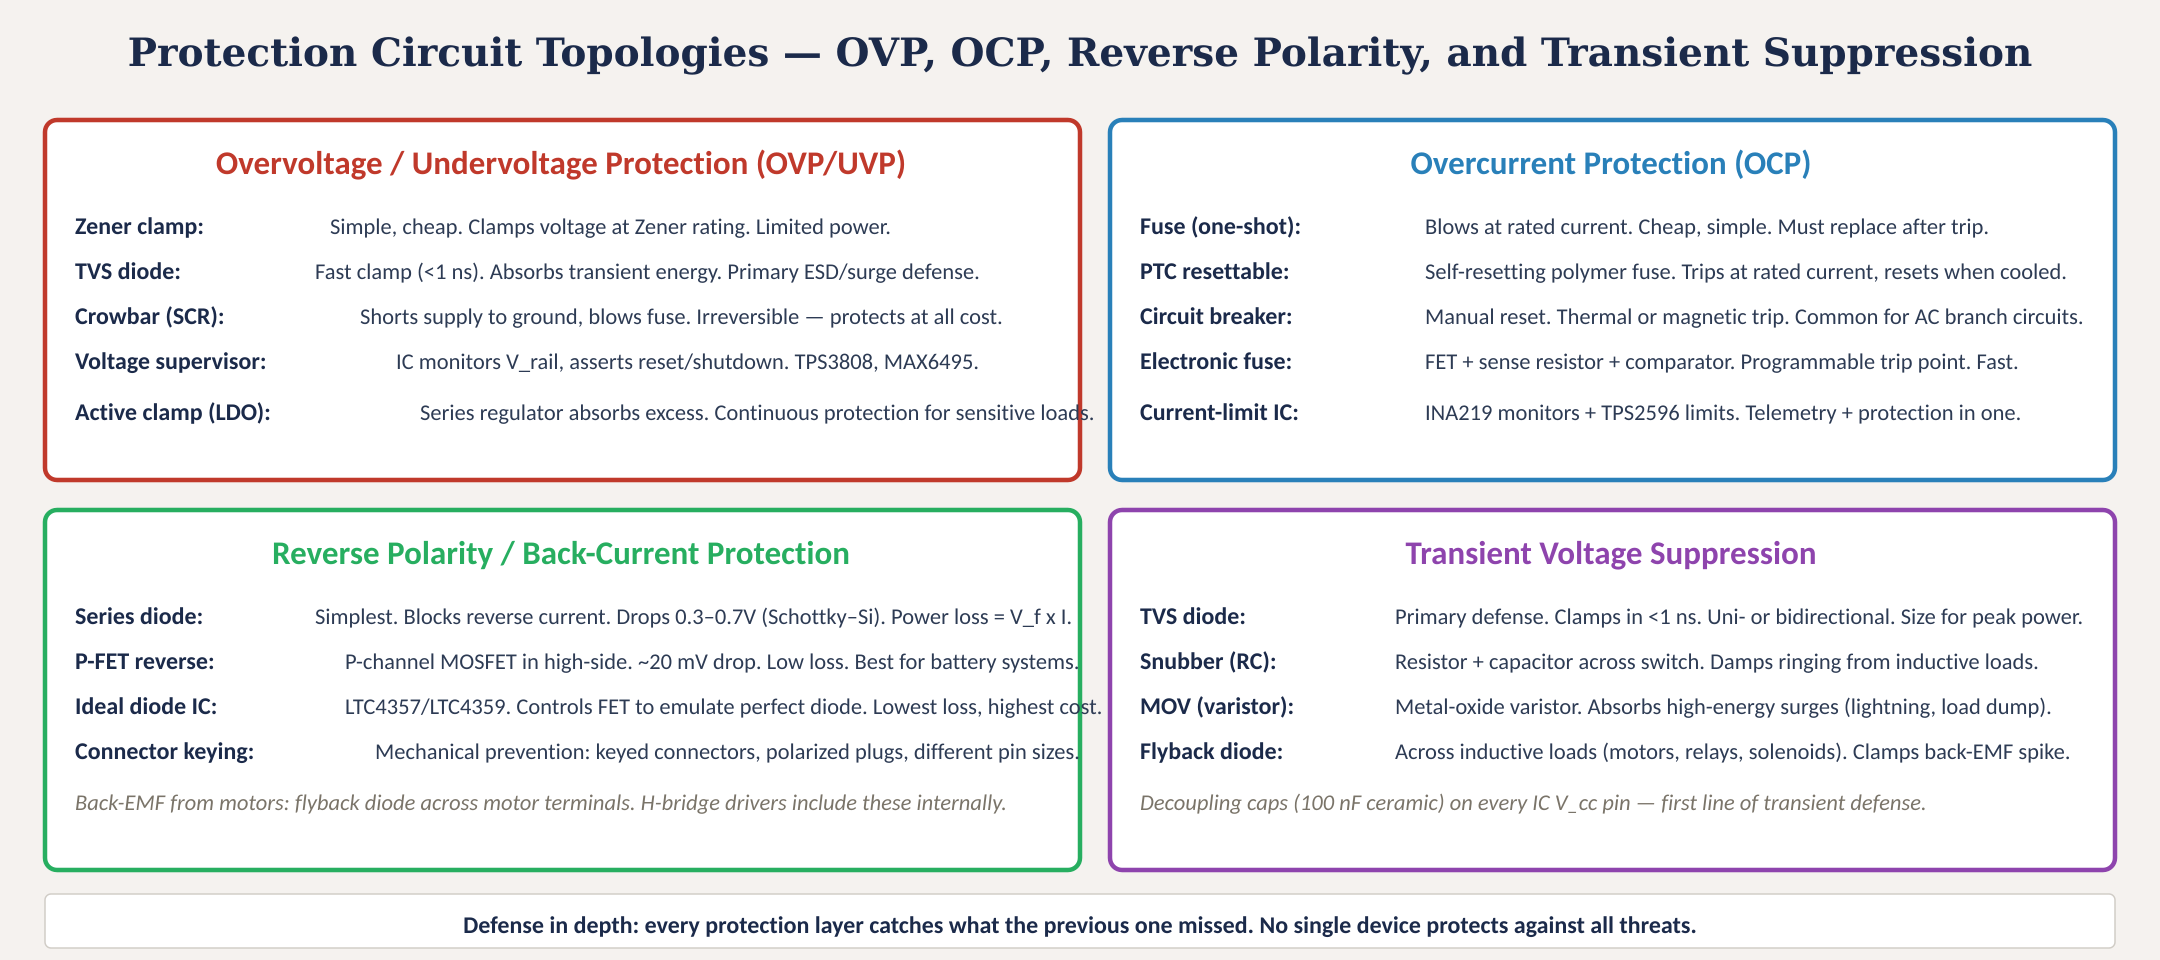
\includegraphics[width=\textwidth]{master_figs/fig_protection_topologies.png}
\caption{Four protection categories: OVP/UVP, OCP, reverse polarity/back-current, and transient suppression with specific device options.}
\label{fig:protection}
\end{figure}


\subsection{Overvoltage and Undervoltage Protection (OVP / UVP)}

\textbf{Overvoltage} pushes components beyond absolute maximum ratings; gate oxide breakdown, latch-up, permanent damage. \textbf{Undervoltage} causes unpredictable behavior: brown-outs, corrupted flash memory, and erratic execution.

\subsubsection{Zener Clamp}
A Zener diode across the supply rail conducts when voltage exceeds its breakdown value, clamping the rail. Simple and cheap but limited by power dissipation ($P = (V_{\text{spike}} - V_Z) \times I$). Select $V_Z$ slightly above your nominal rail (e.g., 5.6\,V Zener for a 5\,V rail).

\subsubsection{TVS Diode}
A Transient Voltage Suppressor; essentially a heavy-duty bidirectional Zener optimized for high peak power. Responds in $<$1\,ns. The primary defense against ESD\index{ESD (electrostatic discharge)}, inductive spikes, and power supply transients. \textbf{Every power input in a professional design has a TVS diode.}

\textbf{Selection}: standoff voltage $\geq$ operating voltage; clamping voltage $<$ component absolute maximum rating. Common series: SMAJ, SMBJ, 1.5KE.

\subsubsection{Voltage Supervisor IC}
Monitors the supply rail and asserts a reset or shutdown signal when voltage is out of range. Does not clamp; it shuts the system down gracefully. Essential for microcontroller brown-out protection. Common: TPS3808 (adjustable OVP/UVP), MAX6495 (OVP with FET control), TLV803 (simple reset).

\subsubsection{Crowbar Circuit}
An SCR (thyristor) fires when voltage exceeds a threshold, shorting the supply to ground and blowing the upstream fuse. \textbf{Irreversible}; the fuse must be replaced. Used as a last resort when the overvoltage source has enough sustained energy to overwhelm a clamp.


\subsection{Overcurrent Protection (OCP)}
\label{sec:ocp}

Every power rail must have current limiting. A short circuit without protection delivers the full energy of the supply into the fault.

\subsubsection{Fuses (One-Shot)}
A fusible element melts at its rated current.\index{inrush current} \textbf{Fast-blow} for sensitive electronics; \textbf{slow-blow} (time-delay) for motor circuits where inrush exceeds steady-state. The fuse must blow \emph{before} the wire or component is damaged. Must be accessible for replacement.

\subsubsection{PTC Resettable Fuses}
Polymer PTC (positive temperature coefficient) devices. Resistance increases dramatically at the trip point, limiting current. Self-resets when cooled. Slower than traditional fuses. Best for USB ports and sensor circuits where the fault is intermittent.

\subsubsection{Electronic Fuses (eFuse)}
A MOSFET in series with the load, controlled by a current-sense amplifier. Programmable trip point, fast response, automatic retry or latched shutdown. Provides current \emph{limiting} (not just cutting); can hold current at a safe level during motor inrush. Common: TPS2596, LTC4368, TPS25944.

\subsubsection{Circuit Breakers}
Thermal or magnetic trip mechanism with manual reset. Common for AC branch circuits (15\,A, 20\,A per NEC). In DC systems, used for battery main disconnects. \textbf{Must be DC-rated}; an AC breaker may not safely interrupt\index{interrupt (ISR)} DC arcs because DC does not cross zero.

\begin{warningbox}[Fuse + Wire Sizing Rule]
The fuse must blow before the wire overheats. This means the fuse rating must be \emph{below} the wire's ampacity. Size them together using NEC Table 310.16 or AWG ampacity charts: the fuse protects the wire, the wire carries the current, and the load defines the requirement.
\end{warningbox}


\subsection{Reverse Polarity and Back-Current Protection}
\label{sec:reverse}

A battery connected backwards forward-biases body diodes of every downstream MOSFET and IC, often destroying the entire board in milliseconds.

\subsubsection{Series Diode}
Simplest approach. A Schottky diode ($\sim$0.3\,V drop) or silicon diode ($\sim$0.7\,V drop) in the positive rail blocks reverse current. Power loss = $V_f \times I_{\text{load}}$. Best for low-current ($<$2\,A) circuits where the voltage drop is acceptable.

\subsubsection{P-Channel MOSFET}
A P-FET in the high-side power path conducts when polarity is correct (body diode initially conducts, pulling gate low, fully enhancing the FET) and blocks when reversed. Voltage drop = $I \times R_{DS(\text{on})}$, typically 10\,--50\,m$\Omega$. At 5\,A with 20\,m$\Omega$: only 0.1\,V drop, 0.5\,W loss. \textbf{Best for battery-powered systems.} Common: Si2301, IRLML6402, DMG2307L.

\subsubsection{Ideal Diode IC}
An IC controlling an external N-FET to emulate a perfect diode with $\sim$20\,mV forward drop. Lowest loss, fastest reverse blocking, highest cost. LTC4357, LTC4359, MAX40200. Also used for OR-ing redundant supplies and solar/battery combining.

\subsubsection{Mechanical Prevention}
Keyed connectors, polarized plugs, and different-sized pins physically prevent reverse connection. The first line of defense. Always use polarized connectors for DC power.


\subsection{Transient Voltage Suppression}
\label{sec:transient}

Every time you switch an inductive load, motor, relay, solenoid, you create a voltage transient. The physics: $V = -L \times dI/dt$. Current cannot change instantaneously in an inductor, so the collapsing magnetic field generates a spike that can reach hundreds of volts from a 12\,V motor.

\begin{figure}[htbp]
\centering
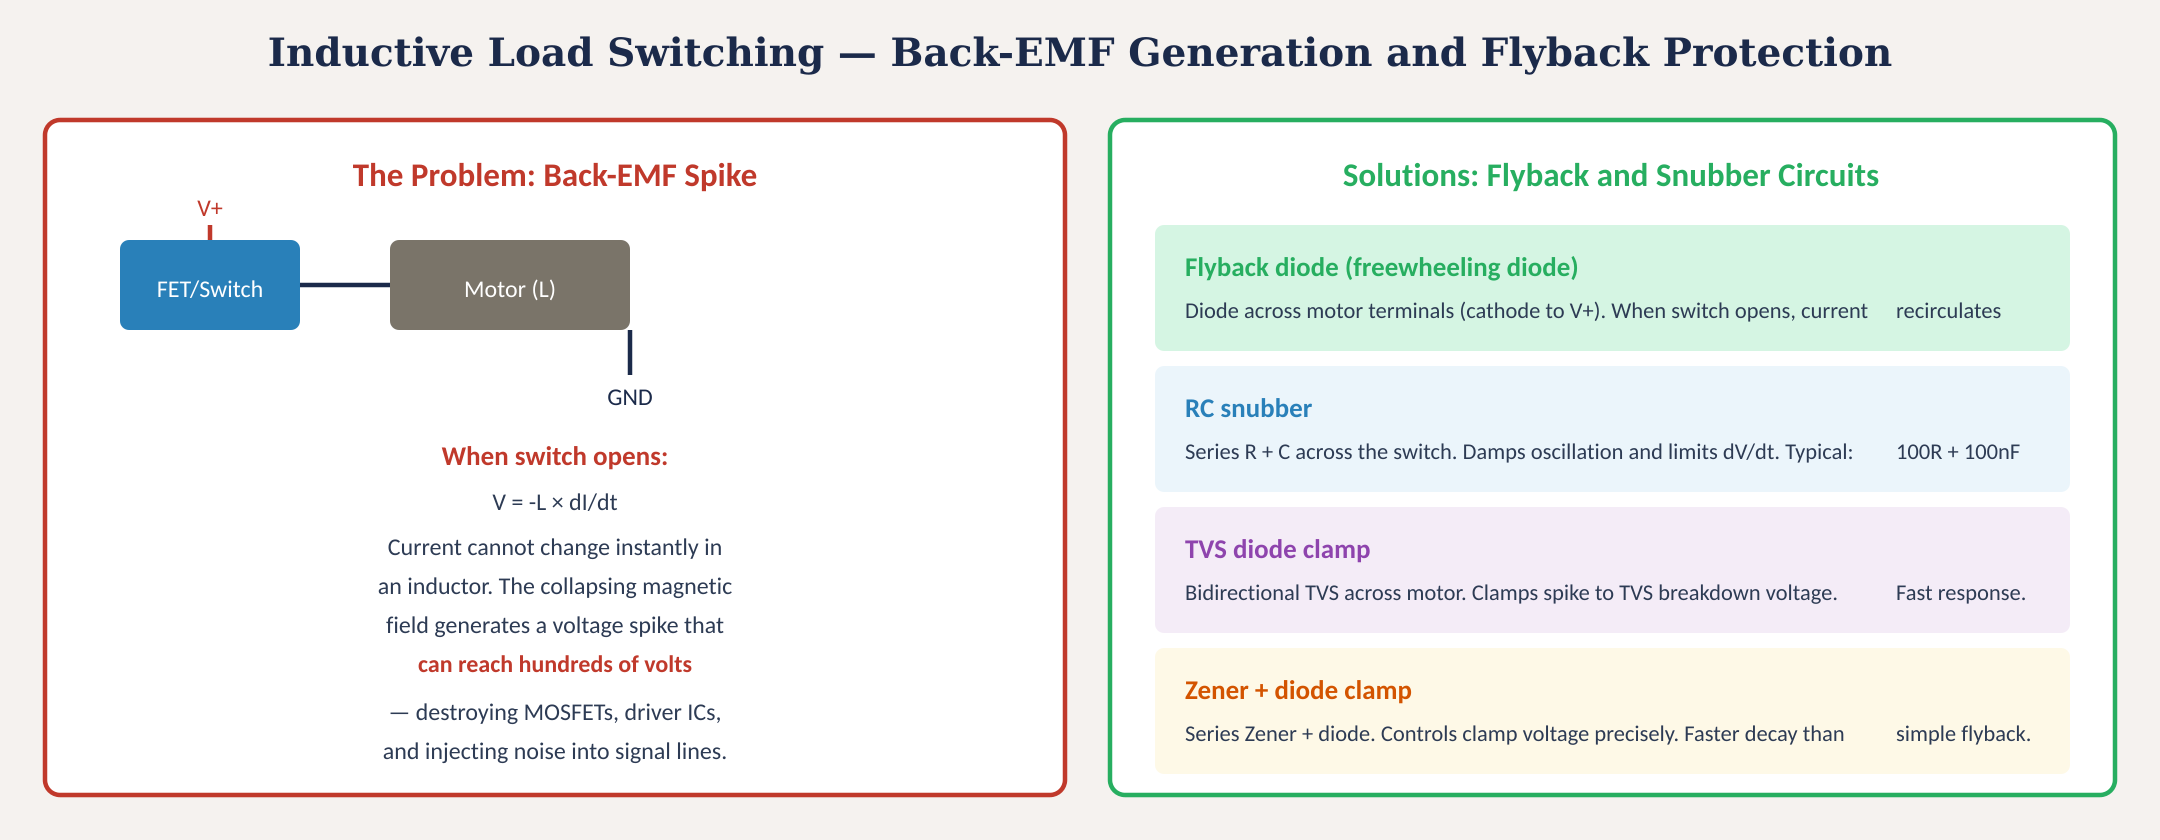
\includegraphics[width=\textwidth]{master_figs/fig_back_emf.png}
\caption{Back-EMF generation from inductive load switching and four protection solutions: flyback diode, RC snubber, TVS clamp, and Zener+diode.}
\label{fig:backemf}
\end{figure}

\subsubsection{Flyback Diode (Freewheeling Diode)}
\textbf{The single most important protection for inductive loads.} A diode across the motor, relay, or solenoid (cathode to V+) provides a current path when the switch opens. Without it, the collapsing field generates a spike that destroys the switching device. Use a fast-recovery or Schottky diode. H-bridge driver ICs include these internally, but if you drive a relay or solenoid with a bare MOSFET, you \textbf{must} add one externally.

\subsubsection{RC Snubber}
A resistor-capacitor network across a switch or relay contact. The capacitor absorbs the initial spike; the resistor dissipates energy and damps oscillation. Typical starting values: 100\,$\Omega$ + 100\,nF for relay contacts. Tune by observing the transient on an oscilloscope.

\subsubsection{TVS Diode (Board-Level)}
Place a TVS across each power rail at the board edge where external cables connect. Absorbs energy from ESD, cable transients, and motor switching spikes propagating through the power bus.

\subsubsection{Decoupling Capacitors}
100\,nF ceramic capacitors on \textbf{every} IC $V_{CC}$ pin, as close to the pin as physically possible. These absorb high-frequency transients before they reach the IC. For power regulators, add bulk capacitance (10\,--100\,$\mu$F) per the datasheet. \textbf{Decoupling is not optional.}


% ══════════════════════════════════════════════════════════════════════
\section{Electromechanical Integration}
\label{sec:mechint}
% ══════════════════════════════════════════════════════════════════════

\begin{figure}[htbp]
\centering
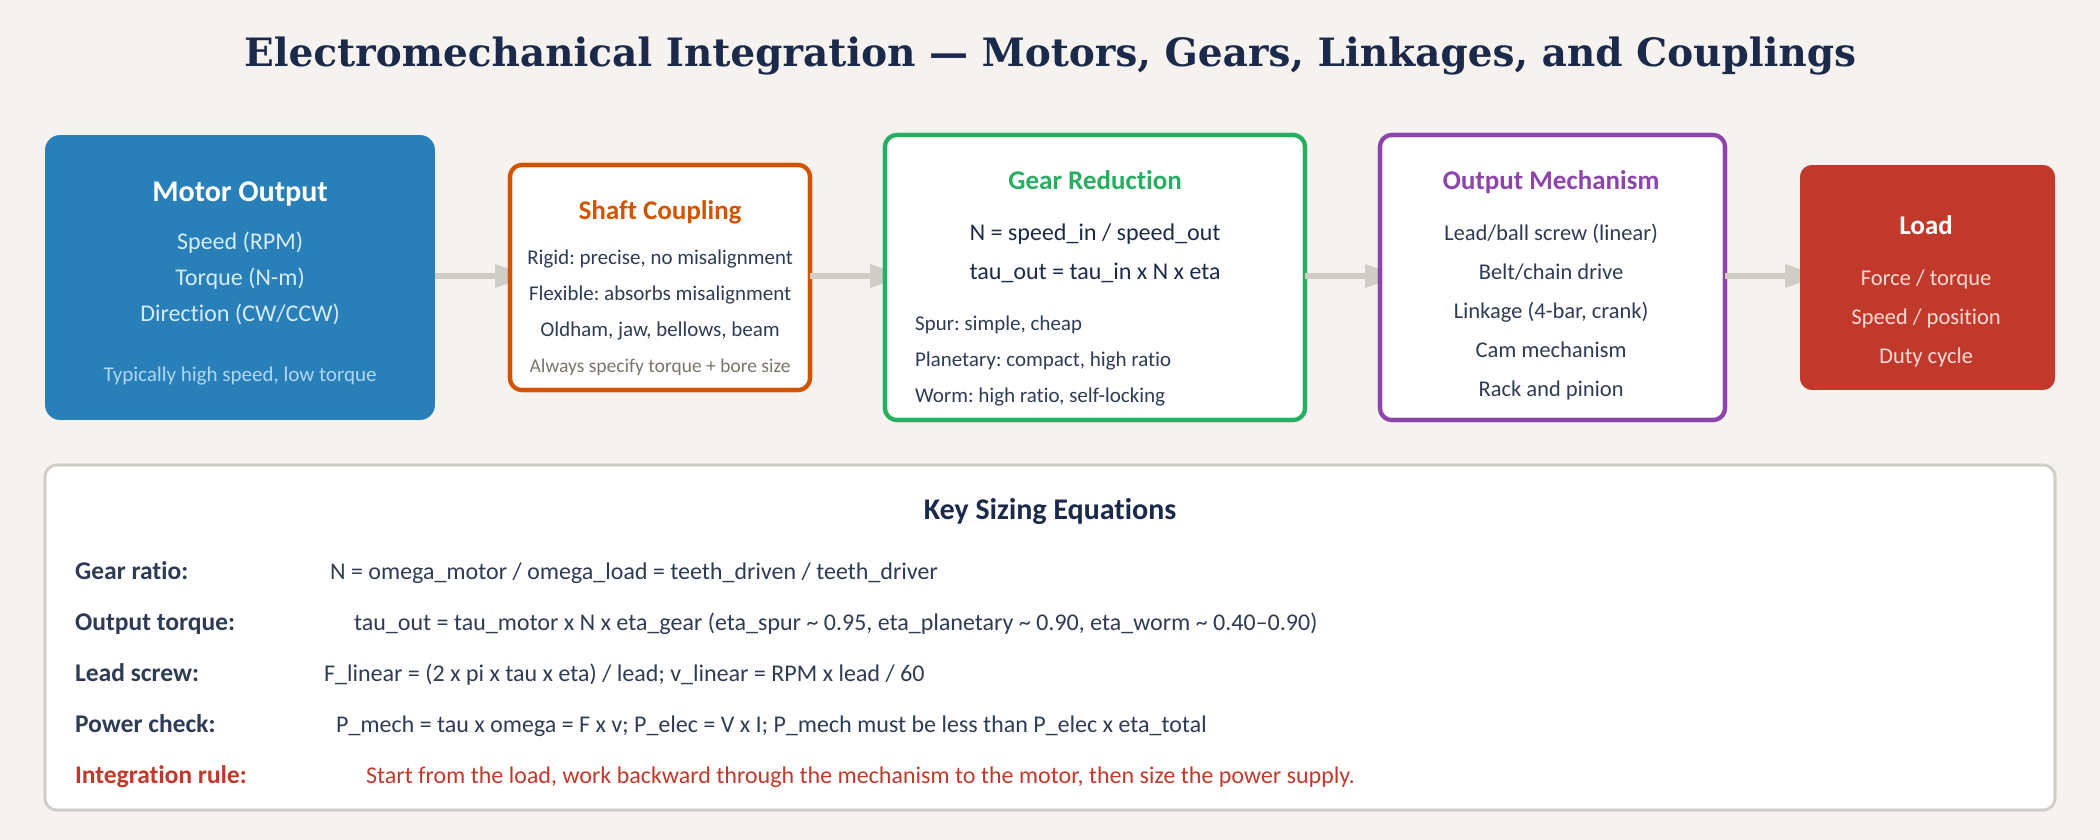
\includegraphics[width=\textwidth]{master_figs/fig_mech_integration.png}
\caption{Motor-to-load power flow through coupling, gear reduction, and output mechanism with key sizing equations.}
\label{fig:mech}
\end{figure}

\subsection{Gear Reduction}

Motors run efficiently at high speed and low torque. Loads typically need the opposite. Gearboxes trade speed for torque:
\begin{equation}
  \tau_{\text{out}} = \tau_{\text{motor}} \times N \times \eta_{\text{gear}}
\end{equation}
where $N$ is the gear ratio ($\omega_{\text{in}} / \omega_{\text{out}}$) and $\eta$ is the gearbox efficiency.

\begin{table}[htbp]
\centering\small
\begin{tabularx}{\textwidth}{l l X}
  \toprule
  \textbf{Type} & \textbf{Efficiency} & \textbf{Characteristics} \\
  \midrule
  Spur & 95--98\% & Simplest, cheapest. External parallel-axis mesh. Available in stock gearmotors. \\
  Planetary & 85--95\%/stage & Compact, coaxial, high torque density. 3:1 to 100:1 per stage. \\
  Worm & 40--90\% & Very high ratios (20:1--300:1) in one stage. Self-locking at high ratios. \\
  \bottomrule
\end{tabularx}
\caption{Gear reduction types and efficiencies.}
\end{table}

\subsection{Output Mechanisms}

\begin{itemize}[leftmargin=1.5em]
  \item \textbf{Shaft couplings}: rigid (zero misalignment tolerance) or flexible (jaw, Oldham, bellows, beam). Beam couplings are the standard for stepper motors\index{stepper motor}.
  \item \textbf{Lead/ball screws}: convert rotary to linear. $F = 2\pi \tau \eta / \text{lead}$. Lead screws are self-locking; ball screws are not.
  \item \textbf{Timing belt\index{timing belt} drives} (GT2, HTD): positive engagement, no slip. Standard for CNC and 3D printers.
  \item \textbf{Linkages} (4-bar, crank-slider, cam): complex output paths. Torque varies through the cycle; size the motor for peak, not average.
\end{itemize}

\begin{keyconceptbox}[Integration Rule]
\textbf{Start from the load and work backward}: calculate the force/torque and speed the load requires $\to$ select the mechanism and gear ratio $\to$ calculate the motor torque $\to$ select the motor $\to$ calculate the current draw $\to$ size the power supply. The power check: $P_{\text{mech}} = \tau \omega = F v$ must be $\leq P_{\text{elec}} \times \eta_{\text{total}}$.
\end{keyconceptbox}


% ══════════════════════════════════════════════════════════════════════
\section{Safety Design Checklist}
\label{sec:checklist}
% ══════════════════════════════════════════════════════════════════════

Every item must be addressed before commissioning:

\begin{enumerate}[leftmargin=1.5em]
  \item Input has reverse polarity protection (P-FET or series diode).
  \item Input has a fuse or electronic current limiter rated for expected peak current.
  \item TVS diode on every power input where external cables connect.
  \item Voltage supervisor on MCU power rail (brown-out reset).
  \item Flyback diode on every inductive load not protected by the driver IC.
  \item Per-rail fusing; each output rail has its own current protection.
  \item 100\,nF decoupling capacitor on every IC $V_{CC}$ pin.
  \item Signal and power grounds separated, joined at a single star point.
  \item Enclosure bonded to earth ground (if using internal AC-DC supply).
  \item All wire gauges sized for their maximum current with appropriate derating.
\end{enumerate}

\begin{keyconceptbox}[Requirements Mapping: From Protection Specs to Shall-Statements]
Protection circuit design generates system requirements:
\begin{itemize}[nosep,leftmargin=1.5em]
\item ``System survives reverse battery'' $\to$ SYS-REQ: The power input shall include reverse-polarity protection limiting leakage to $<$1\,mA.
\item ``Motor inrush must not reset MCU'' $\to$ PWR-REQ: The MCU supply rail shall maintain $\geq$2.7\,V during motor inrush transients up to 15\,A for 100\,ms.
\item ``ESD at user connectors'' $\to$ SYS-REQ: User-accessible interfaces shall withstand $\pm$8\,kV contact discharge per IEC 61000-4-2.
\end{itemize}
Build your power budget spreadsheet \emph{first}, then derive protection requirements from worst-case currents and voltages.
\end{keyconceptbox}


% ══════════════════════════════════════════════════════════════════════
\section{Grounding Architecture}
The grounding strategy is the single most impactful decision for system noise performance:

\textbf{Single-point (star) ground}: all ground returns converge at one physical point. Prevents ground loops (current from one subsystem flowing through another's ground return and creating noise). The star point is typically at the power entry connector. This is the standard for mixed analog/digital systems.

\textbf{Multi-point ground}: each subsystem connects to the nearest ground plane point. Used in high-frequency systems ($>$1\,MHz) where the inductance of long ground wires to the star point would cause resonance. For MEGN~301 projects operating below 1\,MHz: use star grounding.

\textbf{Split ground plane}: on the PCB, use a continuous ground plane under the analog section and a separate continuous ground plane under the digital section, connected at a single point (the star bridge). This prevents digital switching current from flowing under the analog circuits, which would inject noise.

\section{Electromagnetic Compatibility (EMC) Basics}
Every MEGN~301 system is both an EMI source (motors, switching regulators, digital clocks radiate) and an EMI victim (sensors, ADCs, communication lines are susceptible). Basic EMC design rules:

\textbf{Minimize loop areas}: the magnetic field radiated by a current loop is proportional to the loop area. Keep the current path and its return path as close together as possible. A ground plane provides the minimum-area return path for every trace above it.

\textbf{Filter at boundaries}: when a signal enters or leaves the system enclosure, it should pass through a filter (RC low-pass for analog signals, ferrite bead for digital signals, TVS diode for ESD protection). The enclosure boundary is where external EMI enters and internal EMI escapes.

\textbf{Separate noisy and sensitive circuits}: physically separate motor drivers, switching regulators, and high-speed digital circuits from analog sensors and amplifiers. On a PCB: place them on opposite sides. In an enclosure: use separate compartments or shielding barriers.

\textbf{Decouple every IC}: 100\,nF ceramic capacitor within 5\,mm of every IC power pin. This provides local charge storage for fast switching transients, preventing them from propagating through the power bus to other ICs.

\begin{quickrefbox}[Quick Reference: Common Protection Components]
\begin{table}[H]\centering\small
\begin{tabularx}{\linewidth}{l l X}
\toprule
\textbf{Component} & \textbf{Example} & \textbf{Use Case} \\
\midrule
TVS diode & SMBJ12A (12\,V standoff) & ESD and transient voltage clamping on power rails \\
Schottky diode & SS34 (3\,A, 40\,V) & Reverse polarity protection (series); flyback (parallel) \\
P-FET reverse pol.\ & IRLML6402 & Low-loss reverse polarity; $R_{DS(on)} < 50$\,m$\Omega$ \\
PTC fuse (resettable) & MF-R050 (500\,mA) & Signal line overcurrent; auto-resets after fault clears \\
Blade/glass fuse & ATC (automotive) & Main power rail; sized at 125\% of max continuous current \\
eFuse IC & TPS2596 & Programmable current limit, soft-start, fault reporting \\
Varistor (MOV) & 14D471K (470\,V) & AC mains transient suppression \\
Ferrite bead & BLM18PG221 & High-frequency noise filtering on DC power lines \\
\bottomrule
\end{tabularx}
\end{table}
\end{quickrefbox}

\section{Practice Questions}
\label{sec:practice}
% ══════════════════════════════════════════════════════════════════════

\subsection{Conceptual Questions}

\begin{enumerate}[leftmargin=1.5em]
  \item Explain why star-point grounding prevents motor noise from corrupting ADC readings. What happens if motor current returns through a shared ground trace?

  \item A TVS diode has a standoff voltage of 12\,V and a clamping voltage of 19.9\,V at 10\,A. Is this suitable for protecting a 12\,V circuit whose components have a 20\,V absolute maximum rating?

  \item Compare a series Schottky diode versus a P-channel MOSFET for reverse polarity protection at 5\,A. Calculate the power loss for each (Schottky $V_f = 0.3\,V$, P-FET $R_{DS(\text{on})} = 20\,\text{m}\Omega$).

  \item Why must a DC circuit breaker be specifically rated for DC voltage? What is the hazard of using an AC-rated breaker on a DC circuit?

  \item A relay coil has 50\,mH inductance and draws 100\,mA at 12\,V. If the switch opens in 1\,$\mu$s, estimate the back-EMF spike voltage ($V = L \times dI/dt$). Why does this destroy a 60\,V MOSFET?

  \item What is the difference between a crowbar circuit and a TVS diode clamp? When would you use each?

  \item Explain why decoupling capacitors must be placed as close to the IC power pin as possible, not just ``somewhere on the same board.''
\end{enumerate}

\subsection{Application / Scenario Questions}

\begin{enumerate}[resume,leftmargin=1.5em]
  \item Your robot uses a 4S LiPo battery (14.8\,V nominal, 16.8\,V max charge, 12.0\,V cutoff) powering two DC motors (5\,A each continuous, 30\,A each stall), a Raspberry Pi (5\,V, 2.5\,A), and three servos (6\,V, 1\,A each peak). Design the complete power architecture: draw a block diagram showing every rail, regulator, and protection device. Specify part numbers where possible.

  \item Your project team's prototype works perfectly on the bench but fails intermittently in the field. Symptoms: the motor runs fine, but the microcontroller occasionally resets, and analog sensor readings drift by 200\,mV when the motor switches direction. Diagnose the root cause and propose a fix using concepts from this module.

  \item A classmate argues that a flyback diode is unnecessary because ``the motor driver IC already handles back-EMF.'' Under what conditions is the classmate correct? Under what conditions is the classmate dangerously wrong?

  \item Design a protection scheme for a solar panel (18\,V open-circuit, 5\,A short-circuit) charging a 3S LiPo (11.1\,V nominal) that also powers a 12\,V water pump. Include reverse-current blocking, charge control, and load protection.
\end{enumerate}

\subsection{Answers}

\begin{enumerate}[leftmargin=1.5em]
  \item In a shared ground, motor current ($I_M$) flows through the same trace as sensor return current. The trace has resistance $R$, so the sensor sees a ground voltage offset of $V_{\text{noise}} = I_M \times R$. With star-point grounding, motor current returns through its own dedicated conductor, so the sensor ground conductor carries only the small sensor current. The noise voltage on the sensor ground drops from $I_M \times R$ to $I_{\text{sensor}} \times R$, which is typically orders of magnitude smaller.

  \item Yes; the standoff voltage (12\,V) is at or above the operating voltage, so the TVS does not conduct during normal operation. The clamping voltage (19.9\,V) is below the 20\,V absolute maximum, so the TVS clamps before the components are damaged. However, the margin is very tight (0.1\,V). A TVS with a 16.7\,V or lower clamping voltage would provide better margin. Always verify the clamping voltage at the expected peak current, not just the rated value.

  \item Schottky: $P = V_f \times I = 0.3 \times 5 = 1.5\,W$. P-FET: $P = I^2 \times R_{DS} = 25 \times 0.020 = 0.5\,W$. The P-FET dissipates one-third the power. At 5\,A, the Schottky also drops the voltage rail by 0.3\,V, which may push the rail below the minimum operating voltage of downstream components. The P-FET drops only 0.1\,V. For battery-powered systems where efficiency and voltage headroom matter, the P-FET is strongly preferred.

  \item AC current crosses zero 120 times per second (at 60\,Hz), which naturally extinguishes any arc at the breaker contacts. DC current never crosses zero, so a DC arc can sustain indefinitely. An AC-rated breaker's contacts and arc chute may not be designed to extinguish a sustained DC arc, potentially causing the breaker to fail to interrupt the circuit, or worse, catch fire internally.

  \item $V = L \times dI/dt = 0.050 \times (0.100 / 0.000001) = 5000\,V$. This 5\,kV spike (in theory) far exceeds the 60\,V MOSFET's drain-source breakdown voltage. In practice, the MOSFET avalanches and the spike is clamped at the breakdown voltage, but the energy dissipated during avalanche can destroy the device. A flyback diode clamps the spike to approximately $V_{\text{supply}} + V_f \approx 12.7\,V$, well within the MOSFET's rating.

  \item A TVS diode \emph{clamps} the voltage; it conducts just enough to limit the voltage and absorbs the transient energy, then stops conducting when the voltage returns to normal. Operation is non-destructive. A crowbar circuit \emph{shorts} the supply to ground via an SCR, deliberately blowing the upstream fuse. It is destructive (fuse replacement required) but provides guaranteed protection when the overvoltage has enough sustained energy to overwhelm a TVS. Use TVS for transient spikes (ESD, inductive switching); use crowbar for sustained overvoltage from a failed regulator.

  \item Decoupling caps work by providing a low-impedance path for high-frequency transients to bypass the IC rather than entering through the power pins. The trace between the capacitor and the IC pin has inductance proportional to its length. A long trace adds enough inductance to negate the capacitor's effectiveness at high frequencies. Placing the cap within a few millimeters of the pin minimizes this parasitic inductance and keeps the bypass impedance low at the frequencies where transients occur.

  \item Architecture: Battery $\to$ main fuse (80\,A, covers dual motor stall) $\to$ reverse polarity P-FET (IRLML6402 or similar) $\to$ TVS diode (18\,V standoff) $\to$ power distribution bus. Motor rail: direct from battery through individual 40\,A slow-blow fuses per motor, H-bridge drivers with integrated flyback diodes. 5\,V rail: buck converter (e.g., LM2596 or MP1584, 3A rated) from battery bus, with 100\,$\mu$F bulk cap + 100\,nF ceramic decoupling. 6\,V servo rail: buck converter (adjustable output set to 6\,V, 5A rated, TPS54560) with per-servo PTC fuses. BMS: 4S BMS module with 12.0\,V cutoff, 16.8\,V overcharge protection, and cell balancing. Grounds: star-point near main fuse; separate motor ground bus and logic ground bus.

  \item Root cause: ground-coupled motor noise. When the motor reverses direction via the H-bridge, the current transient creates a voltage spike on the shared ground that (a) momentarily shifts the MCU's ground reference, triggering a brown-out reset, and (b) offsets the ADC's reference voltage by 200\,mV, corrupting readings. Fix: (a)~separate motor power ground and MCU signal ground, joining at a star point near the battery; (b)~add a voltage supervisor (TPS3808) on the MCU rail to hold the MCU in clean reset during transients rather than allowing corrupted execution; (c)~add bulk capacitance (470\,$\mu$F) on the MCU's supply rail to absorb the transient; (d)~add a TVS diode on the motor power bus.

  \item The classmate is correct when using a properly rated H-bridge driver IC (like L298N, DRV8871, BTS7960) that includes integrated flyback/freewheeling diodes across the output MOSFETs. These diodes handle the back-EMF from the motor. The classmate is \textbf{dangerously wrong} when: (a)~driving a relay, solenoid, or valve directly from a bare MOSFET or BJT; these loads have no integrated protection; (b)~the motor's back-EMF exceeds the driver's clamping capability; or (c)~using a driver module where the ``protection diodes'' are actually for the logic section, not the motor outputs. \textbf{Rule}: verify in the driver's datasheet that flyback diodes are explicitly rated for the motor's inductive energy.

  \item Solar input: blocking diode (Schottky, e.g., MBR2045) prevents battery discharge through panel at night. MPPT charge controller (e.g., Genasun GV-5 or Victron 75/15) sized for 3S LiPo with 12.6\,V charge termination. Reverse polarity: P-FET on both the solar input and the battery connector. TVS diode (18\,V standoff) on the solar input for transient protection. Load: battery feeds pump through a slow-blow fuse (3\,A for a 2\,A pump). Flyback diode across pump motor terminals. Voltage supervisor monitors battery voltage and disables pump via a load switch when battery drops below 10.5\,V to protect cells. The charge controller's MPPT algorithm ensures maximum solar harvest even as panel voltage varies with sun angle and temperature.
\end{enumerate}


% ══════════════════════════════════════════════════════════════════════


